% FM_P2_CHINESE_SYNC
\documentclass[10pt,conference,letterpaper]{IEEEtran}

\usepackage{fontspec}
\usepackage{xeCJK}
\setmainfont{texgyretermes-regular.otf}[
  BoldFont=texgyretermes-bold.otf,
  ItalicFont=texgyretermes-italic.otf,
  BoldItalicFont=texgyretermes-bolditalic.otf
]
\setCJKmainfont{FandolSong-Regular.otf}[
  BoldFont=FandolSong-Bold.otf,
  ItalicFont=FandolKai-Regular.otf
]
\setCJKsansfont{FandolHei-Regular.otf}
\usepackage{amsmath,amssymb}
\usepackage{graphicx}
\usepackage{booktabs}
\usepackage{tabularx}
\usepackage{array}
\usepackage{multirow}
\usepackage{algorithm}
\usepackage{algpseudocode}
\usepackage{xcolor}
\usepackage{microtype}
\usepackage{cite}
\usepackage{url}
\usepackage{stfloats}
\usepackage{placeins}

\usepackage{amsthm}
\newtheorem{lemma}{引理}
\newtheorem{theorem}{定理}
\providecommand{\FMtodo}[1]{\textbf{[待作者补充：#1]}}
\renewcommand{\proofname}{证明}
\renewcommand{\refname}{参考文献}
\floatname{algorithm}{算法}
\algrenewcommand\algorithmicrequire{\textbf{输入：}}
\algrenewcommand\algorithmicforall{\textbf{对于所有}}
\algrenewcommand\algorithmicfor{\textbf{对于}}
\algrenewcommand\algorithmicif{\textbf{若}}
\algrenewcommand\algorithmicthen{\textbf{则}}
\algrenewcommand\algorithmicelse{\textbf{否则}}
\algrenewcommand\algorithmicdo{\textbf{执行}}
\algrenewcommand\algorithmicend{\textbf{结束}}
\algrenewcommand\algorithmicreturn{\textbf{返回}}

\newcommand{\method}{FedMATRIX-LoRA}
\newcommand{\best}[1]{\textbf{#1}}

\title{FedMATRIX-LoRA：面向资源受限联邦微调的客户端感知矩阵级适配}

\author{\IEEEauthorblockN{匿名作者}}

\begin{document}
\maketitle

\begin{abstract}
联邦微调需要在数据与设备能力异构的客户端之间分配有限的训练资源。对于低秩适配（LoRA），不仅要决定适配器容量，还要决定哪些目标投影接收更新。将投影绑定为不可拆分的 Transformer 块限制了这一位置选择。一项参数预算匹配的受控研究发现，在全部 12 个设置级对比中，无论使用本地还是服务器代理重要性评分，独立矩阵选择的短期验证损失下降量都大于完整层分配。基于这一观察，本文提出 FedMATRIX-LoRA，一种客户端感知的矩阵级适配框架。客户端根据本地梯度画像估计更新优先级，并构建资源可行的矩阵配置；服务器在共享预算与时延目标下协调参与和配置选择。按矩阵聚合结合由此得到的异构更新。条件性平稳性分析刻画了更新偏差与矩阵覆盖的作用。图像分类、语言理解及对话摘要实验评估完整框架，受控研究则考察选择粒度、评分可靠性和各组成部分的贡献。结果支持将重要性引导的矩阵选择作为受限训练预算下有用的适配维度。

\end{abstract}

\begin{IEEEkeywords}
联邦微调，低秩适配，客户端感知矩阵选择，资源异构性
\end{IEEEkeywords}

\section{引言}
基础模型提供可复用的表示，但将其适配到下游应用往往需要不同机构或设备持有的数据。联邦学习使这些数据持有方无须汇集原始样本，就能优化共享模型~\cite{mcmahan2017communication,kairouz2021advances}。对于内存、计算和通信能力有限的客户端，完整参数更新仍然代价高昂。低秩适配（LoRA）保持预训练主干固定，用紧凑的可训练因子表示更新，从而降低这一负担~\cite{hu2022lora}。因此，联邦 LoRA 使协同适配更易实施，但仍需决定每个客户端应利用其可用资源更新哪些适配器参数。

适配器大小本身不能决定训练是否可行。冻结主干、优化器状态以及反向传播时保留的中间激活也需要内存。降低秩会缩小适配器相关状态，却不一定缩短到可训练位置的反向传播路径。Fed-HeLLo 指出这一区别，并报告在激活占主导的设置中，降低秩带来的总内存节省有限~\cite{zhang2025fedhello}。因此，选择可训练位置是秩调整的补充：它改变更新发生的位置，并且在部分适配器执行方式下改变必须保留的激活依赖。我们在固定秩下研究这一位置决策，将目标选择与选中适配器内部的容量分配区分开来。

Transformer 块包含查询、键、值和前馈变换等不同的目标投影。每个投影都可以接收自己的 LoRA 更新。已有位置研究和重要性感知秩分配表明，不同矩阵或层的适配价值不必相同~\cite{hu2022lora,fm_adalora2023}。然而，层级分配将块内候选投影绑定为同一个决策。在有限预算下，选择一个有用的投影可能因此必须同时给同块的其他投影分配容量，并排除别处有用的目标。这引出一个比“不同位置是否重要”更具体的问题：在重要性准则和参数预算固定时，解除完整层绑定能否改善所选的适配配置？

为考察这一问题，我们在 CIFAR100/ViT-base 上比较独立矩阵选择与完整层分配。矩阵级分配从 12 个 Transformer 块中选择 12 个 Q/K/V 目标矩阵；层级分配选择四个块中的全部三个投影。两者均使用秩 8，且可训练参数数量相同。在每一种评分来源下，它们在相同解析式资源限制内最大化同一个画像效用。我们分别评估本地评分与服务器代理评分，涵盖 IID 数据及浓度参数为 $1.0$ 和 $0.1$ 的 Dirichlet 划分。配对配置从初始化或共同预热后的同一适配器出发，进行 20 步本地训练。在前向模型中保留但冻结未选适配器，以隔离可训练子集的影响。第~\ref{sec:fm-granularity-study} 节详述协议。

图~\ref{fig:fm-motivation} 报告矩阵级减去层级的留出验证损失下降量差值。全部 12 个“划分--检查点--评分来源”设置的均值均为正；36 个种子内配对均值中有 35 个为正，每个种子内先对五个客户端求平均。本地和服务器代理重要性评分下均观察到这种改进。这一观察支持独立目标选择作为超越完整层分配的有用适配维度，而不是将收益归因于某一种评分来源。测得的结果是在固定参数预算下的短期损失下降。

\begin{figure}[!t]
  \centering
  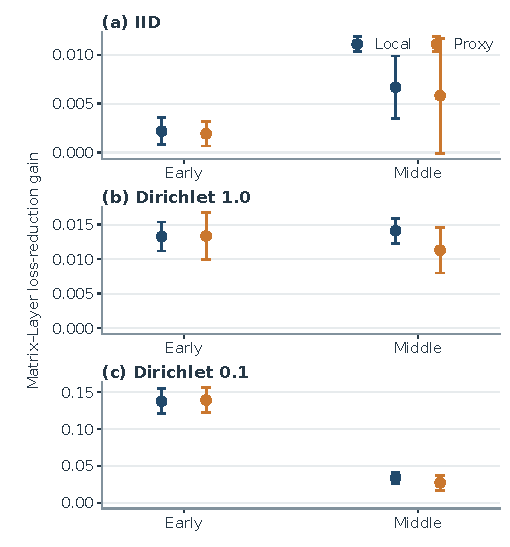
\includegraphics[width=.95\columnwidth]{figures/fig1_p2_granularity_repaired.pdf}
  \caption{矩阵级相对层级选择的验证损失下降增益。在固定协议下，正值表示矩阵级选择更优；误差棒表示种子间标准差。}
  \label{fig:fm-motivation}
\end{figure}

利用这种灵活性，需要在投入训练预算之前评估候选更新。基于梯度和 Fisher 的准则提供了确定可训练参数及 LoRA 层优先级的已有方法~\cite{fm_fish2021,zhang2025fedhello}。这些优先级同时依赖当前模型及评估其损失所用的数据。在联邦系统中，每个客户端已持有定义其本地目标的数据。评估该目标可以提供客户端相关的判断，而不要求服务器另持有画像数据集。Fed-pilot 也将本地及汇总的重要性信息纳入 LoRA 分配~\cite{fm_fedpilot2025}；本文的重点是在块内开放单独的投影选择，并在耦合资源约束下协调这些选择。本地画像是评估机制，动机实验则隔离选择粒度的价值。

但是，高评分子集只有能够训练才有用。内存可行性不仅取决于所选目标的数量，还取决于其位置；客户端计算能力与带宽决定配置能否满足轮次截止时间。即使各项选择单独可行，一起执行时也可能超出共享轮次预算。因此，设计有两个相互关联的要求：在目标矩阵粒度估计更新优先级，并将其转化为可在同一训练轮次协调的客户端可行配置。仅有排序无法解决第二个要求。

为满足这些要求，本文提出 FedMATRIX-LoRA，一种面向资源受限联邦微调的客户端感知矩阵级适配框架。在画像刷新时，每个客户端在当前全局适配器下，使用一个本地小批次评估候选投影的 LoRA 因子。所得评分指导不同矩阵等价成本下的配置，同时满足本地内存和时延限制。服务器在共享预算和同步时延目标下选择客户端配置。客户端训练分配的因子，再按矩阵聚合以更新共享的全局适配器。本地证据指示偏好的目标；资源感知分配决定哪些提议的更新可以共同执行。

本文贡献包括三点：
\begin{itemize}
\item 我们建立面向资源受限联邦微调的重要性引导目标矩阵选择模型，使 Transformer 块内的投影可以独立选择。参数预算匹配的受控研究，在本地与服务器代理两种评分下，以实际短期适配收益说明这一粒度的动机。
\item 我们提出 FedMATRIX-LoRA，将本地矩阵画像、资源可行配置生成、共享预算协调和按矩阵聚合连接起来。客户端可更新不同目标子集，同时对共同的全局适配器作出贡献。
\item 我们给出选择性聚合的条件性平稳性分析，并在图像分类、语言理解和对话摘要任务上评估框架。受控评分和消融研究将各机制与完整系统的性能分别考察。
\end{itemize}

第~\ref{Sec.relatedworks} 节将本文与已有工作比较。第~\ref{sec.model} 节定义系统模型和分配问题。第~\ref{Sec.alg} 节介绍框架及其分析，第~\ref{Sec.evaluation} 节报告评估。第~\ref{Sec.conclusion} 节总结全文。

\section{相关工作}\label{Sec.relatedworks}
\noindent\textbf{参数高效与重要性引导的适配。}
参数高效微调减少适配预训练模型时需要更新的参数。LoRA 通过附着于选定权重矩阵的低秩因子表示更新，QLoRA 则结合量化的冻结主干与可训练适配器~\cite{hu2022lora,dettmers2023qlora}。这些机制处理的是适配开销的不同部分。选择目标子集进一步引入“可训练容量放在哪里”的决策，而不仅是容量大小或存储精度。

重要性感知适配已经表明，有限的参数预算不必均匀分配。AdaLoRA 通过对 SVD 风格的更新参数化进行重要性引导的剪枝，在权重矩阵之间分配非均匀秩预算~\cite{fm_adalora2023}。FISH 使用基于 Fisher 的评分选择稀疏可训练参数掩码~\cite{fm_fish2021}。FedMATRIX-LoRA 在另一分配层次上延续重要性引导的选择：为各联邦客户端选择固定秩目标子集。重要性感知秩分配控制权重更新内部的容量，本文的形式则在异构客户端和轮次级约束下协调可独立选择的目标投影。

\noindent\textbf{异构联邦 LoRA 分配。}
HetLoRA 通过本地秩自剪枝和稀疏加权聚合支持不同的客户端秩，FAH-QLoRA 则联合考虑量化与 LoRA 秩~\cite{cho2024hetlora,gao2025fah}。这些方法根据客户端资源调整容量或数值精度。Fed-HeLLo 指出另一个内存问题：在其研究的激活占主导设置中，降低秩主要影响优化器相关状态，因此部分层训练具有动机~\cite{zhang2025fedhello}。LEGEND 联合配置微调深度和秩分布，明确将可训练位置与资源使用联系起来~\cite{liu2025legend}。因此，目标选择与秩分配是互补而非互斥的维度。

Fed-HeLLo 通过服务器代理评分和几何分配策略考虑层重要性的差异~\cite{zhang2025fedhello}。其评分引导策略将共享评估转化为分配概率，因此客户端可以获得不同的层掩码。FedMATRIX-LoRA 则允许分别选择块内投影，并在客户端数据上评估评分准则。图~\ref{fig:fm-motivation} 的受控对比将矩阵级和层级选择同时应用于两种评分来源，从而区分粒度问题与评分来源问题。它比较的是共同流程中的分配约束，并非对 Fed-HeLLo 的完整复现。

Fed-pilot 是密切相关的重要性引导分配方法。其按块索引的形式结合本地及汇总的梯度信息增益评分、内存约束分配和补偿聚合~\cite{fm_fedpilot2025}。FedMATRIX-LoRA 在块内开放单独的目标投影指示变量，并在内存上限、时延约束和共享轮次预算下跨客户端协调配置。相关差异在于分配决策及其耦合约束，而不只是本地评分或背包求解。

\noindent\textbf{聚合与资源协调。}
FedEx-LoRA 处理聚合低秩因子时的不匹配，LoRA-FAIR 则改进聚合和初始化~\cite{singhal2025fedex,bian2025lorafair}。这些研究关注如何结合本地更新。Oort、FedBalancer 和 PyramidFL 处理异构条件下的参与者选择或训练工作协调~\cite{lai2021oort,shin2022fedbalancer,li2022pyramidfl}。FedMATRIX-LoRA 将可训练目标子集纳入分配给参与客户端的配置。配置生成将本地更新优先级连接到资源可行性，服务器协调决定哪些配置可一起执行。按矩阵收敛性分析刻画由这一过程产生的选择性更新模式。

\section{系统模型与问题定义}\label{sec.model}

\subsection{系统模型与联邦 LoRA 基础}
考虑由一台服务器和 $N$ 个客户端组成的异构联邦 LoRA 微调系统。每个客户端 $i$ 拥有私有本地数据集 $\mathcal{D}_i$、设备端训练显存容量 $M_i^{\max}$（在本实现中对应可用的 GPU 显存）、估计通信带宽 $B_i$ 和异构计算资源。为保护数据隐私，所有本地数据集在整个训练过程中均保留于相应客户端，绝不上传到服务器。服务器初始化预训练主干模型 $\Theta^0$，该模型在联邦微调期间保持冻结，并在通信轮次 $k$ 维护全局 LoRA 适配器参数 $\theta^k$。

令 $n_i=|\mathcal{D}_i|$ 表示客户端 $i$ 的本地训练样本数。联邦 LoRA 微调旨在最小化以下全局目标：
\begin{equation}
F(\theta)=\frac{1}{N}\sum_{i=1}^{N}F_i(\theta),
\end{equation}
其中
\begin{equation}
F_i(\theta)=
\frac{1}{n_i}
\sum_{z\in\mathcal{D}_i}
\ell(\Theta^0,\theta;z),
\label{eq:fl-objective}
\end{equation}
而 $\ell(\cdot)$ 表示使用冻结主干 $\Theta^0$ 和可训练 LoRA 参数 $\theta$ 计算的任务损失。

对于目标线性变换 $W_j\in\mathbb{R}^{d_{\mathrm{out}}\times d_{\mathrm{in}}}$，LoRA 将其更新参数化为
\begin{equation}
\Delta W_j=B_jA_j,
\end{equation}
其中 $A_j\in\mathbb{R}^{r\times d_{\mathrm{in}}}$ 和 $B_j\in\mathbb{R}^{d_{\mathrm{out}}\times r}$ 是秩为 $r\ll \min(d_{\mathrm{in}},d_{\mathrm{out}})$ 的低秩矩阵。

我们将可训练适配器子集视为客户端特定的决策。目标矩阵指查询、键或值等预训练投影；选中目标矩阵意味着更新与其关联的 LoRA 因子，而不是更新冻结的预训练矩阵。每个选中适配器的秩固定且相同，因此配置差异来自目标矩阵的选择。

\subsection{客户端感知的矩阵级 LoRA 分配}
本文在目标矩阵粒度上建模联邦 LoRA 分配。令
\begin{equation}
\mathcal{A}=\{W_1,W_2,\ldots,W_L\}
\end{equation}
表示从主干模型中提取的有序 LoRA 兼容目标矩阵集合。这些矩阵包括 Transformer 块中的查询、键、值、输出和前馈投影矩阵。

对于通信轮次 $k$ 的客户端 $i$，矩阵激活决策由以下二值向量表示：
\begin{eqnarray}
\mathbf m^k_i=[{m}_{i,1}^k,\cdots,{m}_{i,L}^k],
\end{eqnarray}
其中
\begin{eqnarray}
&&{m}_{i,j}^k= \left\{
\begin{aligned}
&1,\mbox{若 $W_j$ 被激活以进行本地训练};\\
&0,\mbox{否则。}
\end{aligned}
\right.
\end{eqnarray}因此，每个激活向量指定客户端 $i$ 在通信轮次 $k$ 中训练的 LoRA 目标矩阵子集。

令 $V_i^k(\mathbf m_i^k)$ 表示客户端 $i$ 的矩阵配置画像效用。它根据当前全局适配器下的本地数据计算，概括了所选更新的估计优先级。我们设 $V_i^k(\mathbf 0)=0$。画像过程见第~\ref{sec:fm-profiling} 节。

若约束同一个 Transformer 块中的所有候选矩阵共用一个选择指示变量，就得到层组分配。

\subsection{资源约束与问题定义}
LoRA 目标矩阵的激活决策决定每个参与客户端的资源消耗。我们分别建模训练成本、训练显存占用和训练时延。

首先，令 $c_i(\mathbf m^k_i)$ 表示矩阵配置 $\mathbf m^k_i$ 对应的标准化训练成本。我们用激活的 rank-8 矩阵数量近似这一成本，即 $c_i(\mathbf m^k_i)=\sum_{j=1}^{L}m_{i,j}^k$。这一标准化计数并非对各矩阵计算量或显存的实际测量；即使秩相同，不同矩阵的开销也可能不同，显存将在下文单独建模。


训练显存消耗同时取决于激活矩阵的数量和位置。对于任意非零配置 \(\mathbf m\)，令
\(\mathcal{J}(\mathbf m)=\{j\mid m_j=1\}\)，且 \(j_{\min}(\mathbf m)=\min\mathcal{J}(\mathbf m)\)。
沿用部分层联邦 LoRA 微调中常用的训练显存分解方式 \cite{zhang2025fedhello}，我们设 \(M_i(\mathbf0)=M_i^{\mathrm{fixed}}\)；对于非零配置，采用
\begin{equation}
M_i(\mathbf m)=M_i^{\mathrm{fixed}}+q_i(r)c_i(\mathbf m)+\sum_{j=j_{\min}(\mathbf m)}^{L}\mu_{i,j},
\label{eq:memory}
\end{equation}
其中，$M_i^{\mathrm{fixed}}$ 表示冻结主干和固定运行时缓冲区占用的显存，$q_i(r)$ 表示每个激活的 rank-\(r\) LoRA 矩阵所需的参数及优化器显存，$\mu_{i,j}$ 表示保留的激活显存。最后一项体现了 Transformer 微调中显存与位置相关的特征：激活更早位置的矩阵需要保留更长的反向传播路径，因此消耗更多激活显存。

客户端 $i$ 的时延由本地计算和通信两部分构成。令 $\gamma_i$ 表示计算系数，$\sigma_i$ 表示每个激活矩阵的通信数据量，$B_i$ 表示可用带宽。其时延为
\begin{equation}
\begin{aligned}
&&T_i^{\mathrm{comp}}(\mathbf m_i)=\gamma_i c_i(\mathbf m_i),\\
&&T_i^{\mathrm{comm}}(\mathbf m_i)=\frac{\sigma_i c_i(\mathbf m_i)}{B_i},\\
&&T_i(\mathbf m_i)=T_i^{\mathrm{comp}}(\mathbf m_i)+T_i^{\mathrm{comm}}(\mathbf m_i).
\end{aligned}
\label{eq:latency-model}
\end{equation}
这些系数定义解析式资源画像；相同的矩阵等价成本不一定对应相同的实测硬件开销。


在通信轮次 $k$，服务器在共享资源预算下联合决定参与客户端及其矩阵配置。令 $S_k$ 表示候选客户端集合，$z_i^k\in\{0,1\}$ 表示客户端 $i$ 是否参与当前轮次，$C^k$ 表示轮次级训练预算，$\tau^k$ 表示当前通信轮次的时延。令 \(\ell_i^{\min}\) 和 \(\ell_i^{\max}\) 分别约束参与客户端 \(i\) 激活矩阵的最小和最大数量，令 \(\lambda>0\) 控制效用与时延的权衡。

\begin{align}
\max_{\{\mathbf m_i^k,z_i^k\},\tau^k}
\quad&
\sum_{i\in S_k}
V_i^k(\mathbf m_i^k)
-\lambda\tau^k
\label{eq:joint-objective}\\
\text{s.t.}\quad&
\sum_{i\in S_k}
c_i(\mathbf m_i^k)
\leq C^k,
\label{eq:joint-budget}\\
&
m_{i,j}^k\leq z_i^k,
\label{eq:participation}\\
&
\ell_i^{\min}z_i^k
\leq
\sum_{j=1}^{L}m_{i,j}^k
\leq
\ell_i^{\max}z_i^k,
\label{eq:bound}\\
&
M_i(\mathbf m_i^k)
\leq M_i^{\max},
\quad
\forall i:z_i^k=1,
\label{eq:joint-memory}\\
&
T_i(\mathbf m_i^k)
\leq
\tau^k
\leq
T_{\max},
\quad
\forall i:z_i^k=1 .
\label{eq:joint-latency}
\end{align}
目标函数在最小化轮次时延的同时，最大化汇总后的客户端相关适配效用。式~\eqref{eq:joint-budget}--\eqref{eq:joint-latency} 分别施加轮次级矩阵等价预算、参与决策一致性、激活矩阵数量上下界、各客户端训练显存上限以及轮次时延上限。特别地，式~\eqref{eq:participation} 和式~\eqref{eq:bound} 共同保证未参与的客户端不选择矩阵，而参与的客户端选择数量在 \(\ell_i^{\min}\) 到 \(\ell_i^{\max}\) 之间的矩阵。


这一问题将客户端层面的可行性与共享轮次预算耦合在一起。我们先在本地构建可行配置，再由服务器协调这些配置来实现求解。

\section{FedMATRIX-LoRA 设计}\label{Sec.alg}
\subsection{框架概述}
FedMATRIX-LoRA 通过客户端相关评估与资源可行分配实现重要性引导的矩阵选择。图~\ref{fig:overview} 区分了这两个作用。客户端利用本地数据对当前适配器进行画像，形成可独立选择目标的配置。服务器在轮次预算和时延目标下协调这些配置。随后，客户端更新被分配的因子，各客户端的贡献按矩阵聚合为下一轮共享适配器。以下小节分别说明评分规则、分配过程、训练协议与条件性分析。

\begin{figure*}[!t]
  \centering
  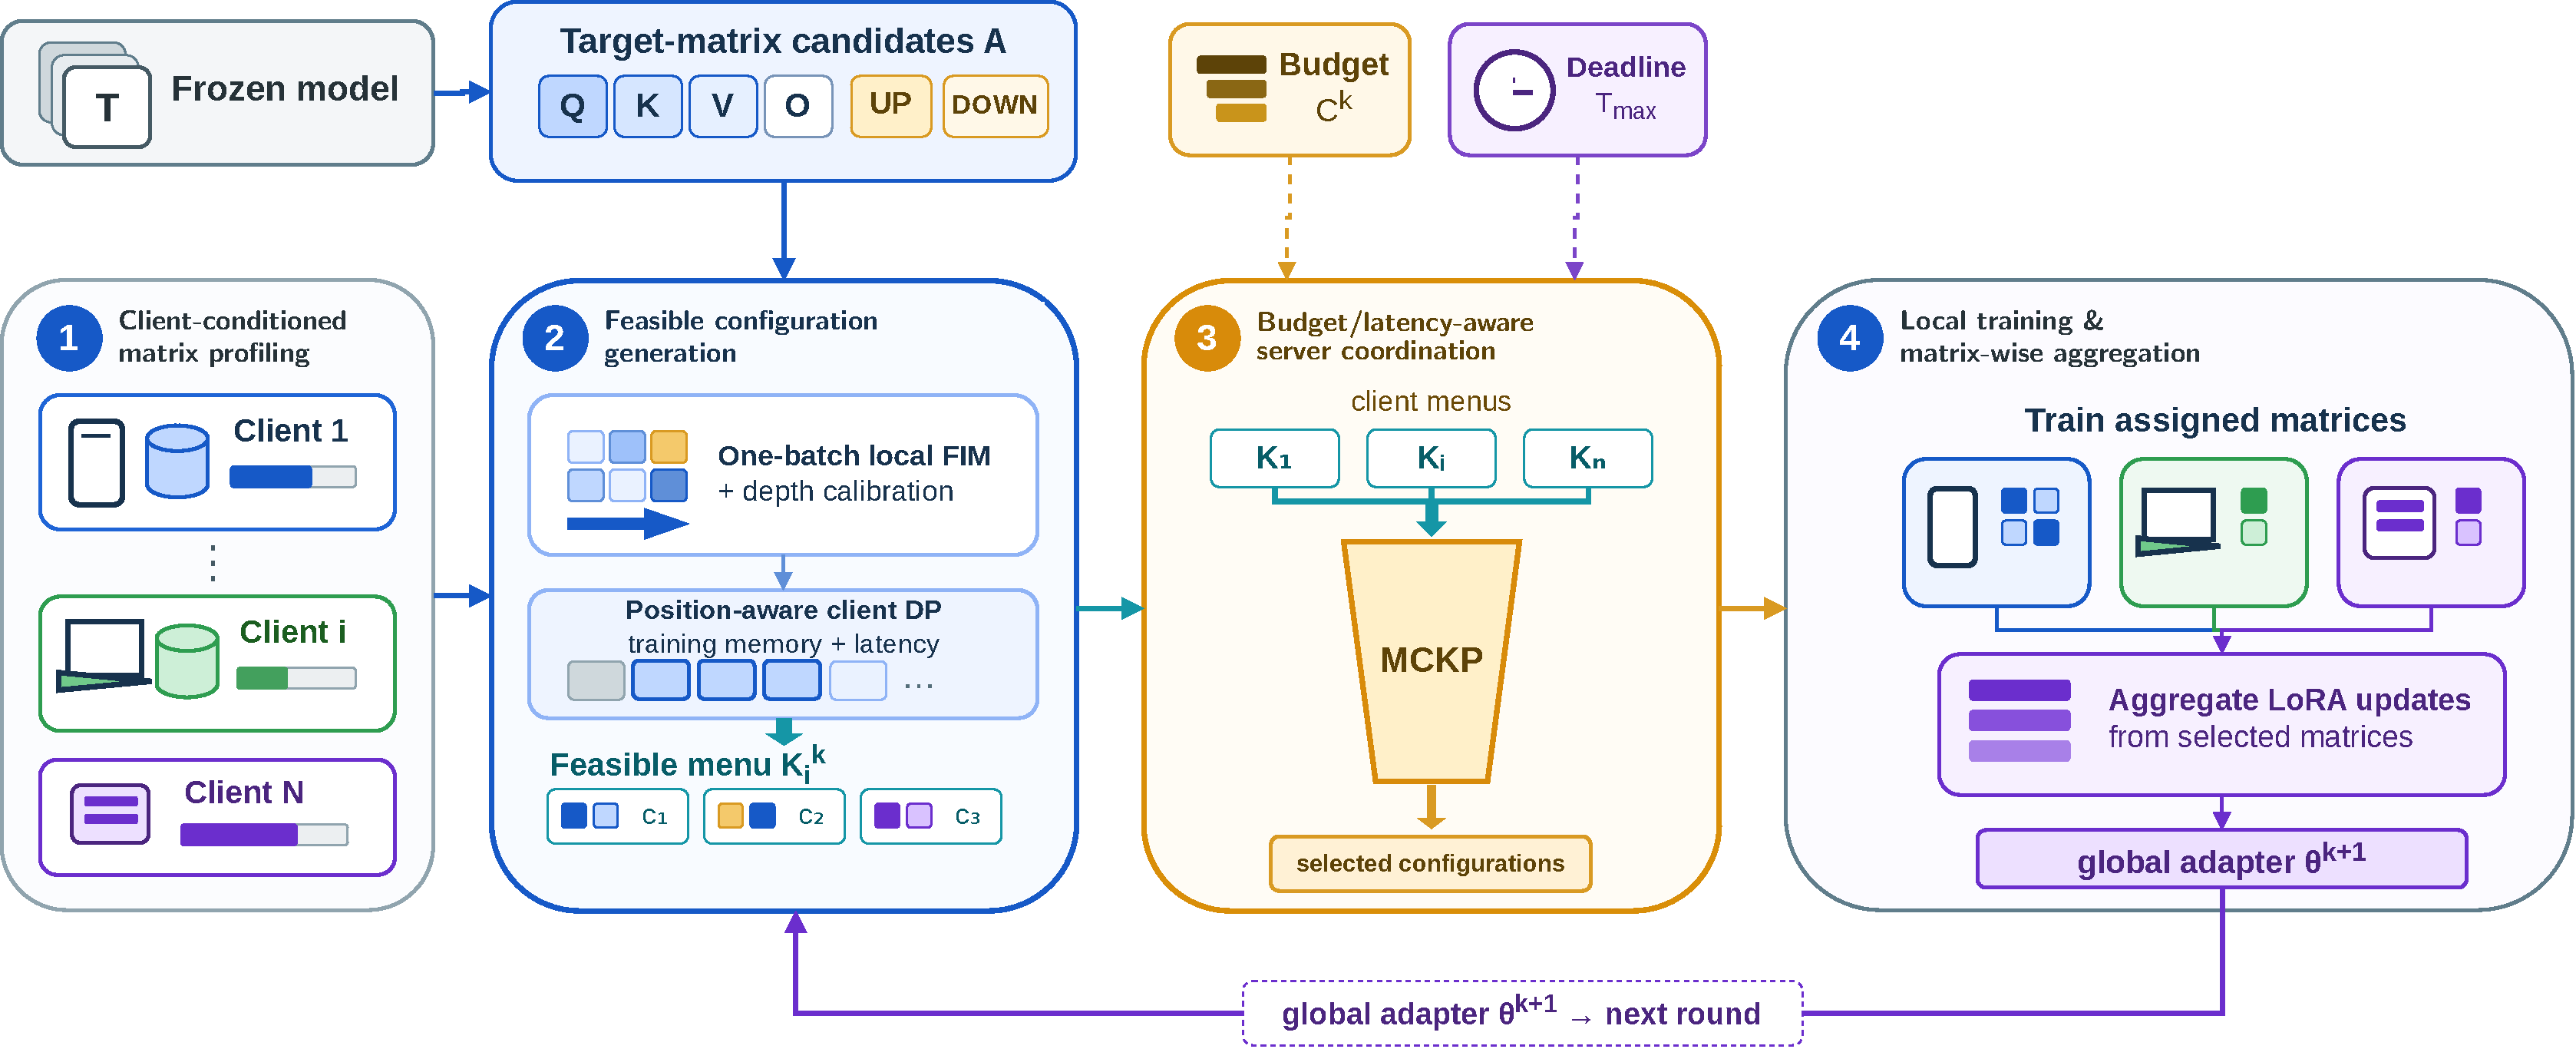
\includegraphics[width=.98\textwidth]{figures/fig2_method_overview_repaired.pdf}
  \caption{FedMATRIX-LoRA 工作流程：客户端相关矩阵画像、本地可行配置生成、预算与时延感知的服务器协调，以及本地训练与按矩阵聚合。}
  \label{fig:overview}
\end{figure*}

\subsection{客户端相关的矩阵画像}\label{sec:fm-profiling}
\noindent\textbf{客户端相关评估。}
动机研究隔离了允许单独选择投影的价值。为了在联邦训练中利用这种灵活性，分配过程需要为每个候选目标提供优先级评分。在共同的全局适配器下，客户端的损失梯度反映其自身样本条件下的参数敏感度。因此，本地评估给出与该客户端目标相关的优先级，而不需要服务器持有画像数据集。配置生成器将这些优先级与资源约束结合，并不把独立的排序直接视为最终训练决策。

\noindent\textbf{单次反向传播的梯度评分。}
基于梯度和 Fisher 的准则已用于选择可训练参数与 LoRA 层~\cite{fm_fish2021,zhang2025fedhello}。我们使用梯度平方准则，在一次反向传播中评估全部候选目标，而不逐个试训练配置。在第 $k$ 轮刷新时，客户端 $i$ 为候选投影附加 LoRA 模块，加载当前全局适配器 $\theta^k$，并计算本地小批次 $\mathcal B_i^k$ 上的平均损失。令 $\theta_j^k$ 表示与目标矩阵 $j$ 关联的 LoRA 因子，其原始评分为
\begin{equation}
 g_{i,j}^k=\sum_{p\in\theta_j^k}
 \left(\nabla_p\mathcal L_i(\theta^k;\mathcal B_i^k)\right)^2.
 \label{eq:fim}
\end{equation}
该评分汇总适配器可训练坐标上批次损失梯度的幅值。平方使各坐标的贡献非负，求和得到块级敏感度，而不是每个参数的均值。在固定参数化下，梯度范数衡量该参数块受到单位范数扰动时的一阶最大敏感度，因此其平方可作为更新优先级信号。计算使用批次平均损失的梯度，所以该评分是受 Fisher 启发的代理指标，而非精确的 Fisher 信息。第~\ref{sec:fm-score-study} 节评估它与短期训练收益的经验关系。

本地样本和当前适配器都进入评分。因此，客户端可以对同一目标给出不同优先级；随着全局模型变化，刷新也允许这些优先级改变。每次画像都评估候选集合，包括该客户端上一轮未更新的目标。因此，下一次分配不只依据其此前活跃的子集。单次反向传播在不对每个候选配置另行优化的情况下提供这些信息。

\noindent\textbf{共享的位置校准。}
原始评分还受到候选位置上的结构性偏好调节。已有部分 LoRA 工作报告，在其研究设置中较深层适配具有有利的性能--资源权衡~\cite{liu2025legend}。我们使用乘性因子：
\begin{equation}
 \widetilde g_{i,j}^k=g_{i,j}^k(1+d_j)^{\rho},
 \label{eq:depth}
\end{equation}
其中 $d_j=(j-1)/(L-1)$ 是有序候选集合中的归一化位置。所评估的日程为 $\rho=1+1.5\mathbb I_{\mathrm{pair}}+\eta$；$\mathbb I_{\mathrm{pair}}$ 表示句子对任务，$\eta=0,1,2$ 分别对应 IID、一般 non-IID 和严重 non-IID 设置。日程由配置固定，而依赖客户端的部分仍是 $g_{i,j}^k$。

共同乘子可以改变某个客户端的排序，但不会取代其数据相关证据，也不会强制所有客户端使用相同掩码。它是辅助偏好，与允许单独选择目标的决策不同。受控粒度研究在每组矩阵--层配对内固定该因子。第~\ref{sec:fm-ablations} 节另行评估移除它对端到端结果的影响。

\noindent\textbf{配置效用与刷新。}
服务器协调需要比较不同客户端提出的配置，因此校准后的评分使用共同的归一化尺度：
\begin{equation}
 G_{\max}^k=\max_{\substack{h\in S_k\\1\le j\le L}}\widetilde g_{h,j}^k,
 \qquad v_{i,j}^k=
 \frac{\widetilde g_{i,j}^k}{\max\{G_{\max}^k,\delta\}}\in[0,1],
 \label{eq:normalization}
\end{equation}
其中 $\delta>0$ 防止除零。共同的除数保留客户端和矩阵之间校准评分的相对大小，并为服务器效用--时延目标设定效用尺度。分配效用为
$V_i^k(\mathbf m_i^k)=\sum_{j=1}^{L}m_{i,j}^kv_{i,j}^k$。
这一可加评分提供可求解的选择目标；它不要求完整训练损失可分解为独立的矩阵损失。本地证据、位置偏好和共同尺度在构建目标时各有作用。

画像在指定刷新轮次之间缓存，并在缺失或应刷新时重新计算。复用避免每次分配决策都额外反向传播；刷新则使评分重新对应当前适配器。原始样本和画像梯度留在本地，协调使用矩阵评分与配置摘要。第~\ref{sec:fm-score-study} 节评估评分提供的排序信息；第~\ref{sec:fm-ablations} 节在完整训练流程中区分评分来源、粒度与校准的影响。

\subsection{资源可行的矩阵分配}\label{sec:fm-allocation}
在固定轮次 \(k\) 中，若不会产生歧义，则省略配置属性和调度变量的轮次上标。客户端 \(i\) 生成的每个可行配置 \(\kappa\) 表示为
\[
\kappa=(V_{i\kappa},c_{i\kappa},T_{i\kappa},M_{i\kappa},\mathbf m_{i\kappa}),
\]
其中，\(V_{i\kappa}\)、\(c_{i\kappa}\)、\(T_{i\kappa}\)、\(M_{i\kappa}\) 和 \(\mathbf m_{i\kappa}\) 分别表示画像适配效用、标准化矩阵等价成本、估计时延、估计训练显存消耗和二值目标矩阵分配。每个客户端上传紧凑的配置菜单 \(\mathcal K_i^k\)。

\noindent\textbf{本地配置。}
在所采用的显存模型下，可行性通过保留激活项取决于选中矩阵的数量和最早选中位置。因此，对于每个数量 $c$，客户端搜索可行的最早位置，保留画像效用最高的配置。令 $Q_{i,e}^k(t)$ 表示从后缀 $\{e,\ldots,L\}$ 中选择 $t$ 个矩阵的最大效用。其递推式及最早选中位置为 $e$ 的配置效用为：
\(Q_{i,e}^k(0)=0\)，\(Q_{i,L+1}^k(t>0)=-\infty\)。
\begin{equation}
 \begin{aligned}
 Q_{i,e}^k(t)&=\max\left\{Q_{i,e+1}^k(t),v_{i,e}^k+Q_{i,e+1}^k(t-1)\right\},\quad t\ge1,
 \\
 \Phi_{i,e}^k(c)&=v_{i,e}^k+Q_{i,e+1}^k(c-1).
 \end{aligned}
 \label{eq:client-dp}
\end{equation}

只保留满足矩阵数量、显存和时延约束的配置。在当前基于数量的时延模型下，成本相同的配置消耗相同的服务器预算并具有相同的时延；因此，每个成本仅保留效用最高的可行配置，已足以供后续协调使用。

\noindent\textbf{服务器协调。}
服务器枚举不同的可行时延阈值 $\tau\le T_{\max}$。对于每个阈值，它移除时延超过 $\tau$ 的配置，再求解剩余的多选择背包问题，即每个客户端至多选择一个配置。令 $H_i(w)$ 表示在预算 $w$ 下，从前 $i$ 个客户端菜单得到的最大效用，其递推式为：

\begin{equation}
 H_i(w)=
 \max_{\kappa\in
 \mathcal K_i^k(\tau)\cup\{\varnothing\}:c_{i\kappa}\le w}
 \left\{
 H_{i-1}(w-c_{i\kappa})
 +
 V_{i\kappa}
 \right\},
 \label{eq:server-dp}
\end{equation}

其中，$\mathcal K_i^k(\tau)$ 是按时延筛选后的菜单，$\varnothing$ 是效用和成本均为零的非活跃选项，且 $H_0(w)=0$。

服务器选择使总效用减去 $\lambda\tau$ 最大的阈值与配置分配。该过程优化的是所定义的画像目标；它的作用是在资源模型下实现客户端相关的选择。算法~\ref{alg:fedmatrix} 概括完整的训练轮次。

\subsection{本地训练与按矩阵聚合}

确定最优配置分配后，服务器将全局适配器 \(\theta^k\) 和选中的矩阵分配一并发送给相应客户端。本地仅更新选中的 LoRA 参数。若下游任务需要任务特定的可训练模块，这些模块与选中的 LoRA 参数联合优化。

由于不同客户端可能更新不同的 LoRA 矩阵子集，聚合过程对每个可训练矩阵独立执行。令 \(\mathcal U_j^k\) 表示返回矩阵 \(j\) 更新的客户端集合，\(\theta_{i,j}^{k+1}\) 表示客户端 \(i\) 对应的本地更新后 LoRA 参数。服务器按矩阵执行客户端等权聚合：

\begin{equation}
 \theta_j^{k+1}
 =
 \begin{cases}
 |\mathcal U_j^k|^{-1}
 \displaystyle\sum_{i\in \mathcal U_j^k}
 \theta_{i,j}^{k+1},
 &
 |\mathcal U_j^k|>0,
 \\[6pt]
 \theta_j^k,
 &
 |\mathcal U_j^k|=0 .
 \end{cases}
 \label{eq:aggregation}
\end{equation}

更新后的全局适配器用于初始化下一轮。由于不同目标矩阵的更新客户端集合可能不同，聚合仅对贡献该矩阵的客户端求平均；若没有客户端返回更新，则保留先前的值。
\begin{algorithm}[t]
\caption{通信轮次 $k$ 中的 \method{}}
\label{alg:fedmatrix}
\footnotesize
\begin{algorithmic}[1]
\Require
全局适配器 \(\theta^k\)，
候选矩阵集合 \(\mathcal A\)，
候选客户端 \(S_k\)，
预算约束 \(C^k\)，
时延上限 \(T_{\max}\)
\Statex \hrulefill
\Statex \textit{客户端相关的矩阵画像与分配：}

\ForAll{\(i\in S_k\)}
    \If{画像缓存不可用或需要刷新}
        \State 在候选矩阵 \(\mathcal A\) 上插入 LoRA 模块
        \State 用一个本地小批次计算矩阵重要性分数 \(g_{i,j}^k\)
        \State 施加位置感知校准，得到 \(\widetilde g_{i,j}^k\)
    \Else
        \State 复用缓存的矩阵重要性分数
    \EndIf
    \State 归一化矩阵效用，得到 \(v_{i,j}^k\)
    \State 通过后缀动态规划生成可行配置菜单 \(\mathcal K_i^k\)
\EndFor

\Statex \hrulefill
\Statex \textit{资源可行的服务器协调：}

\State 初始化最优目标值 \(U^*\leftarrow -\infty\)
\ForAll{不同的可行时延阈值 \(\tau\leq T_{\max}\)}
    \State 移除满足 \(T_{i\kappa}>\tau\) 的配置
    \State 在预算约束 \(C^k\) 下用动态规划求解 MCKP
    \State 计算目标值 \(\sum_i\sum_{\kappa}x_{i\kappa}V_{i\kappa}-\lambda\tau\)
    \If{当前目标值 \(>U^*\)}
        \State 更新最优配置分配
    \EndIf
\EndFor

\Statex \hrulefill
\Statex \textit{本地训练与按矩阵聚合：}
\State 向客户端下发选中的矩阵分配与 \(\theta^k\)
\ForAll{被选中的客户端}
    \State 仅在分配的矩阵上训练 LoRA 参数
\EndFor
\State 执行逐矩阵聚合，得到 \(\theta^{k+1}\)
\State \Return 更新后的全局适配器 \(\theta^{k+1}\)
\end{algorithmic}
\end{algorithm}

\subsection{按矩阵聚合的收敛性}
\label{sec:fm-convergence}
我们分析按矩阵聚合规则所产生的有效更新。在此分析中，$\theta$ 包含 LoRA 参数及联合训练的共享任务模块。令 $P^k$ 表示到第 $k$ 轮所选更新参数块上的投影，这一选择在本地训练前确定。对于公共的正轮次尺度 $\gamma$，将实际聚合方向定义为 $v^k=(\theta^k-\theta^{k+1})/\gamma$。以当前模型、画像信息和已选配置为条件，记这些信息为 $\mathcal H_k$，并定义
\begin{align}
 b^k&=\mathbb E[v^k\mid\mathcal H_k]-P^k\nabla F(\theta^k),\\
 \xi^k&=v^k-\mathbb E[v^k\mid\mathcal H_k].
\end{align}
因此 $\mathbb E[\xi^k\mid\mathcal H_k]=0$，更新可写为
\begin{equation}
 \theta^{k+1}=\theta^k-\gamma\bigl(P^k\nabla F(\theta^k)+b^k+\xi^k\bigr).
\end{equation}
偏差 $b^k$ 涵盖选择性聚合的影响，以及本地优化器更新与所选全局梯度之间的差异。这种表示并未将实验使用的 AdamW 优化器替换为 SGD。

\noindent\textbf{假设。}
假设 $F$ 在相关更新线段上具有 $\beta$-光滑性，并以 $F_{\inf}$ 为下界。假设有效更新误差满足
\begin{equation}
 \mathbb E\|b^k\|^2\le B_{\mathrm{upd}}^2,\qquad
 \mathbb E\|\xi^k\|^2\le S_{\mathrm{upd}}^2.
\end{equation}
此外，假设存在有效矩阵覆盖：对于某个 $0<\alpha_{\mathrm{cov}}\le1$ 和 $\varepsilon_{\mathrm{cov},k}\ge0$，
\begin{equation}
 \mathbb E\|P^k\nabla F(\theta^k)\|^2
 \ge\alpha_{\mathrm{cov}}\mathbb E\|\nabla F(\theta^k)\|^2
       -\varepsilon_{\mathrm{cov},k}.
\end{equation}
这一条件量化了所选参数块覆盖的全局梯度能量。

\begin{theorem}[期望驻点性]
\label{thm:fm-stationarity}
在上述假设下，对于 $0<\gamma\le1/\beta$ 和 $K$ 轮，有
\begin{align}
 \frac1K\sum_{k=0}^{K-1}\mathbb E\|\nabla F(\theta^k)\|^2
 \le{}&\frac{2D_0}{\alpha_{\mathrm{cov}}\gamma K}\\
 &+\frac{B_{\mathrm{upd}}^2+\beta\gamma S_{\mathrm{upd}}^2
              +\bar\varepsilon_{\mathrm{cov}}}{\alpha_{\mathrm{cov}}},\nonumber
\end{align}
其中，对于固定的初始化，$D_0=F(\theta^0)-F_{\inf}$，且
$\bar\varepsilon_{\mathrm{cov}}=K^{-1}\sum_k\varepsilon_{\mathrm{cov},k}$。
\end{theorem}
在固定分析轮数下，若取 $\gamma=c/\sqrt K\le1/\beta$，并且误差上界和覆盖常数在所分析运行中一致，则优化项和噪声项为 $O(K^{-1/2})$。剩余项由有效更新偏差和未覆盖的梯度能量控制。该结果刻画的是平均驻点性，而非最优测试准确率。

客户端选择的贡献可以进一步明确。令 $n_j=|\mathcal U_j|>0$、$g_{i,j}=\nabla_jF_i(\theta)$、$g_j=N^{-1}\sum_i g_{i,j}$，以及 $\zeta_j^2=N^{-1}\sum_i\|g_{i,j}-g_j\|^2$。
\begin{lemma}[按矩阵选择的偏差]
\label{lem:fm-selection-bias}
对于任意更新客户端集合 $\mathcal U_j$，
\begin{equation}
 \left\|\frac1{n_j}\sum_{i\in\mathcal U_j}g_{i,j}-g_j\right\|^2
 \le\left(\frac N{n_j}-1\right)\zeta_j^2.
\end{equation}
\end{lemma}
该界将聚合偏差与每个目标矩阵的参与程度和梯度异构性联系起来。证明见附录~\ref{app:fm-convergence}。



\section{实验}\label{Sec.evaluation}
我们在主基准设置上评估完整框架，并利用受控研究区分选择粒度、评分可靠性与组成部分的作用。资源效率比较采用文中所述的解析式客户端资源画像。

\subsection{评估设置}
我们在 CIFAR100 \cite{krizhevsky2009cifar} 上评估图像分类，在 GLUE \cite{wang2019glue} 的 MNLI、QNLI、QQP 和 SST-2 上评估语言理解，并在 SAMSum \cite{gliwa2019samsum} 上评估对话摘要。

表~\ref{tab:setup} 给出了主干模型、数据划分、轮数和 rank-8 矩阵成本预算；每轮有十个客户端。分类任务采用均等随机 IID 划分，或 $\alpha=1.0$、$0.1$ 的 Dirichlet non-IID 划分。SAMSum 使用连续分配的长度排序数据块构造严重偏斜，使用随机分配的长度排序数据块构造轻度偏斜。

\begin{table*}[t]
\centering
\caption{评估设置。Non-IID \(x\) 表示 Dirichlet \(\alpha=x\)；Len-M/S 表示轻度/严重的长度偏斜；斜线分隔的预算按数据划分顺序排列。}
\label{tab:setup}
\setlength{\tabcolsep}{4.0pt}
\begin{tabular}{@{}llllrrl@{}}
\toprule
数据集 & 任务 & 主干模型 & 数据划分 & 轮数 & 累计预算 & 指标 \\
\midrule
CIFAR100 & 图像分类 & ViT-base \cite{dosovitskiy2021vit} & IID, Non-IID 1.0/0.1 & 180 & 7,200/12,000 & 准确率 \\
MNLI & 语言推断 & DeBERTa-v3-large \cite{he2021deberta} & IID, Non-IID 1.0 & 50 & 9,500 & 准确率 \\
QNLI & 句子对分类 & RoBERTa-base \cite{liu2019roberta} & IID, Non-IID 1.0 & 80 & 4,800/7,200 & 准确率 \\
QQP & 复述句分类 & DeBERTa-v3-large \cite{he2021deberta} & IID, Non-IID 1.0 & 50 & 9,500 & 准确率 \\
SST-2 & 情感分类 & RoBERTa-base \cite{liu2019roberta} & IID, Non-IID 1.0 & 80 & 7,200 & 准确率 \\
SAMSum & 对话摘要 & OPT-1.3B \cite{zhang2022opt} & IID, Len-M, Len-S & 40 & 10,000 & Rouge-L \\
\bottomrule
\end{tabular}
\end{table*}

\begin{figure*}[t]
  \centering
  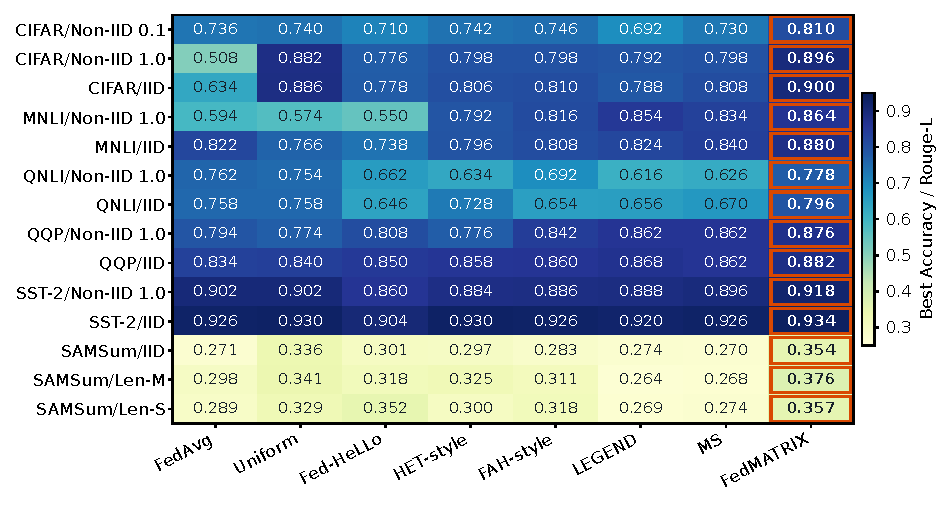
\includegraphics[width=.62\textwidth]{figures/fig3_main_results.pdf}
  \caption{14 种设置下的最佳任务指标。方框标记每行的最大值；SAMSum 使用 Rouge-L，其余各行使用准确率。}
  \label{fig:matrix}
\end{figure*}

\begin{table}[t]
\centering
\caption{系统与训练画像。}
\label{tab:resource-profile}
\setlength{\tabcolsep}{3.6pt}
\begin{tabular}{@{}ll@{}}
\toprule
控制项 & 报告的配置 \\
\midrule
客户端数 & 10 \\
训练显存预算 & 40/25/15 GB；比例 6:3:1 \\
计算系数 & 每个 rank-8 矩阵等价量 0.8--2.0 s \\
带宽 & 5--50 MB/s \\
LoRA 秩／画像 & 8／一个本地小批次 \\
本地训练上限 & 一个 epoch，最多 50 个小批次步 \\
优化器 & AdamW \\
批大小／学习率 & 1--32／\(10^{-5}\)--\(10^{-4}\) \\
默认时延上限 & 每轮 200 s \\
\bottomrule
\end{tabular}
\end{table}

联邦运行使用 NVIDIA A800-SXM4-80GB GPU。表~\ref{tab:resource-profile} 给出解析式客户端资源画像与训练设置。主要对比使用种子 2024，且共享数据划分和资源抽样。新增的评分与消融研究分别报告其种子集合和数据划分。累计训练成本 \(\overline C^K=\sum_{k=1}^{K}\sum_i c_i(\mathbf m_i^k)\) 不包含画像开销。时间曲线累计的是式~\eqref{eq:latency-model} 中的解析式时延，而非端到端墙钟时间。

%Measured wall-clock times are reported separately in Section~V-E.




对于分类任务，我们报告最终和最佳准确率；对于 SAMSum，报告 ROUGE-L，不将两种指标混合求平均。

我们将 \method{} 与代表性基线比较，包括同构 LoRA 训练（FedAvg-LoRA）\cite{mcmahan2017communication,hu2022lora}、均匀矩阵分配（Uniform）、逐层分配（Fed-HeLLo）\cite{zhang2025fedhello}、层组启发式分配（MS）、异构秩分配（LEGEND \cite{liu2025legend} 和 HETLoRA-style \cite{cho2024hetlora}），以及量化和秩的联合分配（FAH-QLoRA-style）\cite{gao2025fah}。这些基线代表不同的适配粒度和资源分配策略，可与本文客户端感知的矩阵调度进行全面对比。为保证公平，所有方法使用相同的主干模型、数据划分、通信轮次、本地训练设置和评估协议。


\subsection{任务性能与资源效率}
图~\ref{fig:matrix} 比较 14 种评估设置下观察到的最佳任务指标。如图~\ref{fig:matrix} 所示，在覆盖 IID 与异构数据划分的全部 CIFAR100、GLUE 和 SAMSum 设置中，\method{} 始终排名第一。与异构秩和量化基线相比，\method{} 也取得显著更高的峰值性能。例如，在 MNLI IID 中，HETLoRA-style 和 FAH-QLoRA-style 分别达到 $0.796$ 和 $0.808$，而 \method{} 达到 $0.880$。在 CIFAR100 IID 中，三者相应的准确率分别为 $0.806$、$0.810$ 和 $0.900$，展示了完整框架在所报告评估协议下的性能。

图~\ref{fig:budget-curves} 中的预算--质量轨迹，刻画了累计矩阵等价成本增加时获得的性能。结合表~\ref{tab:time-to-quality} 中匹配目标的对比，它们量化了完整框架的资源权衡。

\begin{figure*}[!t]
  \centering
  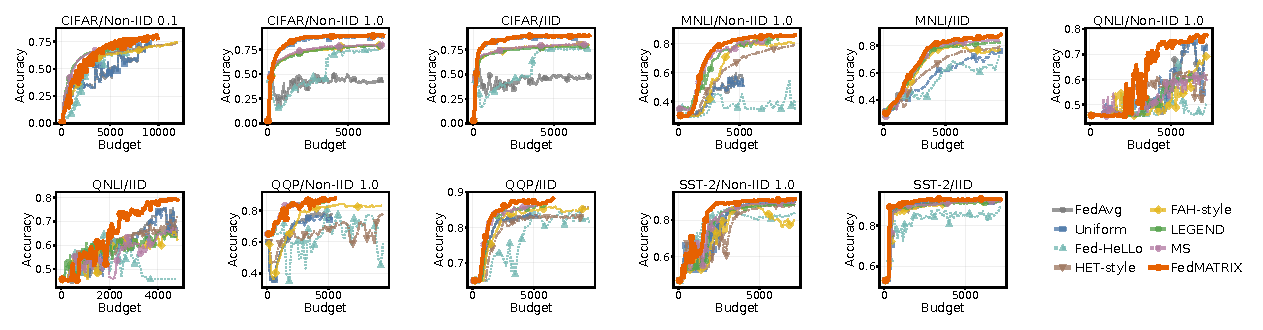
\includegraphics[width=.92\textwidth]{figures/fig4_budget_curves.pdf}
  \caption{11 种分类场景的预算--质量轨迹；突出显示 \method{}。}
  \label{fig:budget-curves}
\end{figure*}

\begin{figure*}[!t]
  \centering
  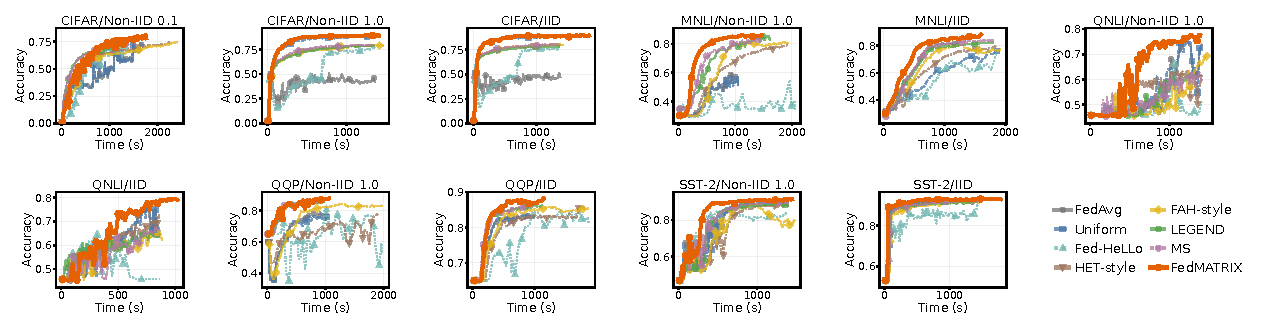
\includegraphics[width=.92\textwidth]{figures/fig5_time_curves.pdf}
  \caption{全部 11 种分类场景的模型估计时间--质量轨迹，使用与图~\ref{fig:budget-curves} 相同的解析式客户端画像。}
  \label{fig:time-curves}
\end{figure*}

图~\ref{fig:time-curves} 报告在相同解析式客户端资源画像下，以累计模型估计时延为横轴的对应轨迹。表~\ref{tab:time-to-quality} 中的匹配目标结果概括了模型估计时间节省；这些数值不同于端到端实测运行时间。

我们还比较达到分类任务峰值准确率所需的资源。表~\ref{tab:time-to-quality} 报告 \method{} 相对于达到相同目标时资源消耗最少的基线，在累计成本和模型估计时间方面的节省（$\Delta\overline C$ 和 $\Delta T$）。在全部 $11$ 种分类场景中，\method{} 使用的资源更少，累计预算和模型估计经过时间的中位节省分别为 $41.3\%$ 与 $42.3\%$，表明它在多种工作负载下持续具有更高的资源效率。

\begin{table}[!t]
\centering
\caption{达到各最强基线的峰值准确率所需的资源；正的节省率有利于 \method{}。}
\label{tab:time-to-quality}
\setlength{\tabcolsep}{2.2pt}
\resizebox{\columnwidth}{!}{%
\begin{tabular}{@{}llrrr@{}}
\toprule
场景 & 参照方法 & 目标值 & $\Delta\overline C$ (\%) & $\Delta T$ (\%) \\
\midrule
CIFAR / Non-IID 0.1 & FAH-style & .746 & +53.9 & +59.4 \\
CIFAR / Non-IID 1.0 & Uniform & .882 & +42.9 & +42.4 \\
CIFAR / IID & Uniform & .886 & +54.4 & +48.3 \\
MNLI / Non-IID 1.0 & LEGEND & .854 & +5.6 & +27.7 \\
MNLI / IID & MS & .840 & +33.2 & +42.3 \\
QNLI / Non-IID 1.0 & FedAvg & .762 & +0.7 & +3.2 \\
QNLI / IID & FedAvg & .758 & +17.4 & +3.2 \\
QQP / Non-IID 1.0 & LEGEND & .862 & +14.9 & +21.7 \\
QQP / IID & LEGEND & .868 & +41.3 & +44.2 \\
SST-2 / Non-IID 1.0 & FedAvg & .902 & +44.4 & +45.2 \\
SST-2 / IID & HET-style & .930 & +47.8 & +38.5 \\
\bottomrule
\end{tabular}
}
\end{table}

\subsection{选择粒度的受控研究}
\label{sec:fm-granularity-study}
图~\ref{fig:fm-motivation} 的研究将可训练子集决策与评分数据来源区分开来。我们在 CIFAR100/ViT-base 上使用 36 个 Q/K/V 候选、五个客户端、IID 和 Dirichlet-$1.0/0.1$ 划分，以及种子 2024--2026。形成客户端数据前，从训练划分中预留独立的服务器代理样本池和预热数据划分。每个客户端留出 100 个样本用于验证。本地画像使用 16 个客户端训练样本；Proxy 对五个互不重叠、各含 16 个样本的代理批次求平均。两个检查点分别是适配器初始化，以及在独立预留集上预热 100 步后的结果，并非两个联邦通信轮次。

对于每个客户端、检查点和评分来源，矩阵选择器在资源可行的 12 目标子集中最大化画像评分。层选择器枚举所有四块组合，在每个被选块中将 Q/K/V 绑定。两者使用相同的来源评分、深度因子、资源限制和秩 8；LoRA 与共同训练的分类头参数数量相同。在所用资源模型下，全部 360 条方法记录均可行。未选中的适配器保留在前向模型中但被冻结，且每个配置都从相同的验证损失出发。20 步 AdamW 训练使用学习率 $10^{-3}$、每组配对内相同的数据顺序和受控随机状态。这一协议衡量匹配初始函数后的适配效果，而不是删除适配器带来的内存收益。

矩阵--层差值先在每个种子内对五个客户端求平均，再跨三个种子汇总。全部 12 个设置级均值为正；36 个种子内配对均值中有 35 个、180 个客户端级配对中有 161 个偏向矩阵级选择。完整数值汇总见附录~\ref{app:fm-p2-details}。由于两种评分来源下都观察到改进，该研究支持解除完整层绑定，而不要求本地评分优于代理评分。深度校准沿用与方法相同的划分相关日程，并在每组配对内固定。

\subsection{评分可靠性}\label{sec:fm-score-study}
接下来考察可加效用是否能为所选矩阵--层配对之外的配置提供有用的排序信息。在 CIFAR100 研究的每个客户端与检查点上，我们评估原有的 12 个不同的可行配置，其中包含评分引导和随机子集。每个配置均使用 12 个秩为 8 的目标、相同训练长度和匹配的初始适配器。结果指标是在留出本地样本上的训练前损失减去训练后损失。粒度对比新增的层级配置不加入这个候选池。

原始评分和深度校准评分的 Spearman 相关系数分别在每个客户端--检查点候选池内计算。先在每个种子内对五个客户端系数求平均，再报告三个种子的均值和样本标准差。统计使用配对随机状态修复后的训练结果；配置身份和评分值均保持不变。

\newcommand{\FMAdepthMin}{0.657}
\newcommand{\FMAdepthMax}{0.876}
\newcommand{\FMApositive}{90}
\newcommand{\FMAtotal}{90}
\newcommand{\FMAassociationSentence}{这些设置级的正相关支持在本受控协议中使用画像效用为配置确定优先级。}
\begin{table}[t]
\centering
\caption{客户端内部的配置排序可靠性。数值为先对客户端求平均、再跨三个种子计算的 Spearman 系数均值 $\pm$ 样本标准差。预热表示共同的 100 步检查点。}
\label{tab:fm-score-reliability}
\small
\setlength{\tabcolsep}{3pt}
\begin{tabular}{@{}llcc@{}}
\toprule
数据划分 & 状态 & 原始评分 & 校准评分 \\
\midrule
IID & 初始化 & $0.688\pm0.114$ & $0.746\pm0.067$ \\
IID & 预热 & $0.595\pm0.094$ & $0.657\pm0.070$ \\
Dir. $1.0$ & 初始化 & $0.792\pm0.012$ & $0.841\pm0.042$ \\
Dir. $1.0$ & 预热 & $0.556\pm0.141$ & $0.664\pm0.136$ \\
Dir. $0.1$ & 初始化 & $0.885\pm0.028$ & $0.772\pm0.028$ \\
Dir. $0.1$ & 预热 & $0.801\pm0.023$ & $0.876\pm0.036$ \\
\bottomrule
\end{tabular}
\end{table}


校准评分的六个设置级平均相关系数介于 \FMAdepthMin{} 与 \FMAdepthMax{} 之间；\FMAtotal{} 个客户端--检查点系数中有 \FMApositive{} 个为正。\FMAassociationSentence{} 表~\ref{tab:fm-score-reliability} 对相同训练结果报告原始和校准评分，从而区分梯度信号的信息量与位置因子的作用。本实验考察短期配置排序；下一个消融在完整联邦训练中评估这些设计。

\subsection{矩阵级适配的消融}\label{sec:fm-ablations}
我们使用 Dirichlet-$1.0$ 划分下的 SST-2/RoBERTa-base 隔离三个组成部分。Full 与三个变体比较：Server-Proxy 用仅从预留训练样本构建的共享代理评分替代本地评分；Layer-Level 保留本地评分，但绑定同一块中的 Q/K/V 选择；No-Depth 仅移除位置乘子。在每个种子内，所有变体使用相同的私有数据与代理数据划分、秩 8、本地优化器设置、候选客户端协议、资源限制和 80 轮训练长度。实际选中的客户端及目标子集仍是分配结果。三个种子为 2024--2026，每次运行消耗累计 7,200 的矩阵等价预算。该受控研究具有自己的代理预留集，与历史主对比实验分开报告。

\begin{table}[t]
\centering
\caption{累计矩阵等价预算为 7,200 时的 SST-2 组成部分消融。验证准确率以百分比表示，报告三个种子的均值 $\pm$ 样本标准差。最佳值为每次运行中的峰值。粗体表示各指标列的最大均值。}
\label{tab:fm-ablations}
\small
\setlength{\tabcolsep}{4pt}
\begin{tabular}{@{}lcc@{}}
\toprule
变体 & 最终准确率 & 最佳准确率 \\
\midrule
Full & $\mathbf{90.60}\pm0.72$ & $90.87\pm0.50$ \\
Server-Proxy & $90.47\pm0.81$ & $90.80\pm0.87$ \\
Layer-Level & $90.07\pm1.33$ & $90.73\pm0.42$ \\
No-Depth & $90.47\pm0.61$ & $\mathbf{90.93}\pm0.42$ \\
\bottomrule
\end{tabular}
\end{table}

\begin{figure*}[t]
\centering
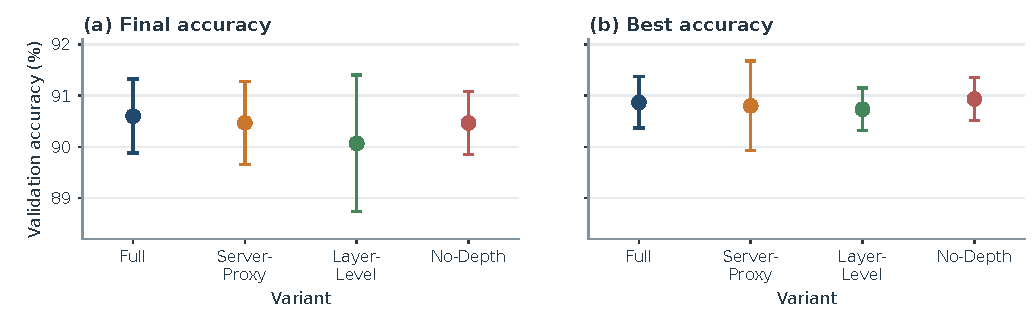
\includegraphics[width=.85\textwidth]{figures/fig6_ablation_accuracy_repaired.pdf}
\caption{四种消融变体在三个种子上的最终与最佳验证准确率。误差棒表示标准差；所有变体消耗相同的累计矩阵预算。}
\label{fig:fm-ablation-budget}
\end{figure*}

表~\ref{tab:fm-ablations} 同时报告最终与最佳准确率，图~\ref{fig:fm-ablation-budget} 展示其种子间变化。Full 的最终均值最高，分别比 Server-Proxy、Layer-Level 和 No-Depth 高 $0.13$、$0.53$ 和 $0.13$ 个百分点。在这一设置中，绑定完整层造成的最终均值变化最大，与短期粒度研究互为补充。这些差异相对于不同运行之间的变化幅度较小。本地评估和代理评估的观测均值接近，而 No-Depth 的最佳均值略高，为 $90.93\%$。因此，消融将目标粒度的贡献与评分来源和校准较小的终点影响区分开来，而不把完整框架在主基准上的收益归因于某一个组成部分。

\FloatBarrier
\section{结论}\label{Sec.conclusion}
FedMATRIX-LoRA 在异构客户端资源条件下，将单独的 LoRA 目标投影视为可选适配单元。动机受控研究表明，在测试的设置均值中，无论使用本地评分还是服务器代理评分，矩阵级选择都比完整层绑定带来更大的短期收益。框架利用本地数据评估优先级，构建可行配置，并在按矩阵聚合前于共享预算下协调其执行。条件性分析将由此产生的选择性更新与有效更新偏差及矩阵覆盖联系起来。主基准实验与受控消融评估这一设计的互补方面：完整框架的性能和资源权衡，以及评分与分配机制的作用。这些结果共同说明，重要性引导的目标选择是资源受限联邦适配中值得采用的一个维度。

\appendices
\section{按矩阵聚合的证明}
\label{app:fm-convergence}
\begin{proof}[定理~\ref{thm:fm-stationarity} 的证明]
以 $\mathcal H_k$ 为条件，令 $a=P^k\nabla F(\theta^k)$，且
$\bar v=\mathbb E[v^k\mid\mathcal H_k]=a+b^k$。
由于更新仅作用于 $P^k$ 所选的参数块，光滑性给出
\begin{align}
 \mathbb E[F(\theta^{k+1})\mid\mathcal H_k]
 \le{}&F(\theta^k)-\gamma\langle a,\bar v\rangle\\
 &+\frac{\beta\gamma^2}{2}
 \left(\|\bar v\|^2+\mathbb E[\|\xi^k\|^2\mid\mathcal H_k]\right).\nonumber
\end{align}
利用 $2\langle a,\bar v\rangle=\|a\|^2+\|\bar v\|^2-\|b^k\|^2$，并由
$\gamma\le1/\beta$ 舍去非正项
$-\gamma(1-\beta\gamma)\|\bar v\|^2/2$。取全期望可得
\begin{align}
 \mathbb E F(\theta^{k+1})\le{}&\mathbb E F(\theta^k)
 -\frac\gamma2\mathbb E\|P^k\nabla F(\theta^k)\|^2\\
 &+\frac\gamma2B_{\mathrm{upd}}^2
 +\frac{\beta\gamma^2}{2}S_{\mathrm{upd}}^2.\nonumber
\end{align}
对 $k$ 求和后，损失项望远镜相消。由 $F$ 的下界得到
\begin{equation}
 \frac1K\sum_k\mathbb E\|P^k\nabla F(\theta^k)\|^2
 \le\frac{2D_0}{\gamma K}+B_{\mathrm{upd}}^2+\beta\gamma S_{\mathrm{upd}}^2.
\end{equation}
再应用覆盖条件，并除以 $\alpha_{\mathrm{cov}}$。
\end{proof}

\begin{proof}[引理~\ref{lem:fm-selection-bias} 的证明]
令 $d_i=g_{i,j}-g_j$，$w_i=\mathbf1\{i\in\mathcal U_j\}/n_j$。
由于 $\sum_i d_i=0$，选择偏差等于 $\sum_i(w_i-1/N)d_i$。
Cauchy--Schwarz 不等式给出
\begin{align}
 \left\|\sum_i(w_i-1/N)d_i\right\|^2
 &\le\sum_i(w_i-1/N)^2\sum_i\|d_i\|^2\\
 &=(1/n_j-1/N)N\zeta_j^2,
\end{align}
即所需界。对于完整的有效偏差，令其余本地更新差异为 $r=b-s$；当没有客户端更新某参数块时，令相应的选择偏差块为零。于是 $\|b\|^2\le2\|s\|^2+2\|r\|^2$。后一项包含本地漂移、优化器效应和任何本地模型不匹配；仅凭选择偏差引理无法约束它。
\end{proof}


\section{完整的受控研究结果}
\label{app:fm-p2-details}
表~\ref{tab:fm-p2-complete} 列出参数预算匹配的粒度研究中全部“划分--检查点--评分来源”条件。每个数值先在种子内对五个客户端的配对差值求平均，再报告三个种子的均值和样本标准差。初始化与 100 步预热检查点被明确区分。这些是损失差值，不是准确率百分点。
\begin{table*}[t]
\centering
\caption{20 步留出验证损失下降量中完整的矩阵级减层级差值。数值为三个种子内客户端均值的均值 $\pm$ 样本标准差。}
\label{tab:fm-p2-complete}
\small
\begin{tabular}{@{}llcc@{}}
\toprule
数据划分 & 检查点 & 本地评分 & 代理评分 \\
\midrule
IID & 初始化 & $+0.00219\pm0.00140$ & $+0.00191\pm0.00125$ \\
IID & 预热 & $+0.00669\pm0.00319$ & $+0.00582\pm0.00591$ \\
Dir. $1.0$ & 初始化 & $+0.01328\pm0.00211$ & $+0.01335\pm0.00335$ \\
Dir. $1.0$ & 预热 & $+0.01411\pm0.00179$ & $+0.01130\pm0.00330$ \\
Dir. $0.1$ & 初始化 & $+0.13752\pm0.01708$ & $+0.13907\pm0.01669$ \\
Dir. $0.1$ & 预热 & $+0.03412\pm0.00757$ & $+0.02726\pm0.01002$ \\
\bottomrule
\end{tabular}
\end{table*}


\section{评分来源对照}
\label{app:fm-source-control}
原有的评分来源对照单独于粒度动机实验汇总。Local 评估各客户端自己的数据；Local-Mean 对五个客户端的原始评分向量求平均；Proxy 对五个互不重叠的服务器代理批次求平均。Local 在每个客户端使用 16 个样本，Proxy 总计使用 80 个样本。它们使用相同的校准、固定矩阵数量、训练长度和留出评估协议。表~\ref{tab:fm-source-control} 报告与评分研究使用相同随机状态修复后，Local 减去各对照方法的损失下降量差值。正负差值均予保留。主要动机来自每种评分来源内部的矩阵--层比较；本表刻画评分来源之间的互补对比。
\begin{table*}[t]
\centering
\caption{配对随机状态修复后的完整评分来源对照。数值为留出验证损失下降量中 Local 减对照方法的差值，附三个种子的样本标准差。}
\label{tab:fm-source-control}
\small
\begin{tabular}{@{}llcc@{}}
\toprule
数据划分 & 状态 & Local 减 Proxy & Local 减 Local-Mean \\
\midrule
IID & 初始化 & $-0.00011\pm0.00038$ & $-0.00011\pm0.00038$ \\
IID & 预热 & $-0.00125\pm0.00274$ & $-0.00243\pm0.00338$ \\
Dir. $1.0$ & 初始化 & $-0.00040\pm0.00076$ & $-0.00029\pm0.00056$ \\
Dir. $1.0$ & 预热 & $-0.00090\pm0.00122$ & $-0.00028\pm0.00068$ \\
Dir. $0.1$ & 初始化 & $-0.00440\pm0.00467$ & $-0.00049\pm0.00816$ \\
Dir. $0.1$ & 预热 & $-0.00050\pm0.00015$ & $-0.00141\pm0.00133$ \\
\bottomrule
\end{tabular}
\end{table*}


\FloatBarrier
\begin{thebibliography}{99}
\bibitem{zhang2022opt}
S. Zhang \emph{et al.},
``OPT: Open pre-trained transformer language models,''
\emph{arXiv preprint arXiv:2205.01068}, 2022.

\bibitem{dosovitskiy2021vit}
A. Dosovitskiy \emph{et al.},
``An image is worth 16x16 words: Transformers for image recognition at scale,''
in \emph{Proceedings of the International Conference on Learning Representations (ICLR)}, 2021.

\bibitem{mcmahan2017communication}
B. McMahan, E. Moore, D. Ramage, S. Hampson, and B. A. y Arcas,
``Communication-efficient learning of deep networks from decentralized data,''
in \emph{Proceedings of the 20th International Conference on Artificial Intelligence and Statistics (AISTATS)}, 2017, pp. 1273--1282.

\bibitem{kairouz2021advances}
P. Kairouz \emph{et al.},
``Advances and open problems in federated learning,''
\emph{Foundations and Trends in Machine Learning}, vol. 14, nos. 1--2, pp. 1--210, 2021,
doi: 10.1561/2200000083.

\bibitem{hu2022lora}
E. J. Hu, Y. Shen, P. Wallis, Z. Allen-Zhu, Y. Li, S. Wang, L. Wang, and W. Chen,
``LoRA: Low-rank adaptation of large language models,''
in \emph{Proceedings of the International Conference on Learning Representations (ICLR)}, 2022.

\bibitem{cho2024hetlora}
Y. J. Cho, L. Liu, Z. Xu, A. Fahrezi, and G. Joshi,
``Heterogeneous LoRA for federated fine-tuning of on-device foundation models,''
in \emph{Proceedings of the 2024 Conference on Empirical Methods in Natural Language Processing}, 2024, pp. 12903--12913,
doi: 10.18653/v1/2024.emnlp-main.717.

\bibitem{gao2025fah}
Z. Gao, Z. Zhang, Y. Guo, and Y. Gong,
``Federated adaptive fine-tuning of large language models with heterogeneous quantization and LoRA,''
in \emph{Proceedings of IEEE Conference on Computer Communications (INFOCOM)}, 2025, pp. 1--10,
doi: 10.1109/INFOCOM55648.2025.11044641.

\bibitem{zhang2025fedhello}
Z. Zhang, P. Liu, J. Xu, and R. Hu,
``Fed-HeLLo: Efficient federated foundation model fine-tuning with heterogeneous LoRA allocation,''
\emph{IEEE Transactions on Neural Networks and Learning Systems}, vol. 36, no. 10, pp. 17556--17569, 2025,
doi: 10.1109/TNNLS.2025.3580495.

\bibitem{li2021moon}
Q. Li, B. He, and D. Song,
``Model-contrastive federated learning,''
in \emph{Proceedings of the IEEE/CVF Conference on Computer Vision and Pattern Recognition (CVPR)}, 2021, pp. 10713--10722,
doi: 10.1109/CVPR46437.2021.01057.

\bibitem{dettmers2023qlora}
T. Dettmers, A. Pagnoni, A. Holtzman, and L. Zettlemoyer,
``QLoRA: Efficient finetuning of quantized LLMs,''
in \emph{Advances in Neural Information Processing Systems}, vol. 36, 2023, pp. 10088--10115.

\bibitem{houlsby2019adapters}
N. Houlsby, A. Giurgiu, S. Jastrzebski, B. Morrone, Q. de Laroussilhe, A. Gesmundo, M. Attariyan, and S. Gelly,
``Parameter-efficient transfer learning for NLP,''
in \emph{Proceedings of the 36th International Conference on Machine Learning}, vol. 97, 2019, pp. 2790--2799.

\bibitem{li2021prefix}
X. L. Li and P. Liang,
``Prefix-tuning: Optimizing continuous prompts for generation,''
in \emph{Proceedings of the 59th Annual Meeting of the Association for Computational Linguistics and the 11th International Joint Conference on Natural Language Processing (Volume 1: Long Papers)}, 2021, pp. 4582--4597,
doi: 10.18653/v1/2021.acl-long.353.

\bibitem{zhang2023fedpetuning}
Z. Zhang, Y. Yang, Y. Dai, Q. Wang, Y. Yu, L. Qu, and Z. Xu,
``FedPETuning: When federated learning meets the parameter-efficient tuning methods of pre-trained language models,''
in \emph{Findings of the Association for Computational Linguistics: ACL 2023}, 2023, pp. 9963--9977,
doi: 10.18653/v1/2023.findings-acl.632.

\bibitem{chen2022fedtune}
J. Chen, W. Xu, S. Guo, J. Wang, J. Zhang, and H. Wang,
``FedTune: A deep dive into efficient federated fine-tuning with pre-trained transformers,''
\emph{arXiv preprint arXiv:2211.08025}, 2022.

\bibitem{che2023fedpeptao}
T. Che, J. Liu, Y. Zhou, J. Ren, J. Zhou, V. Sheng, H. Dai, and D. Dou,
``Federated learning of large language models with parameter-efficient prompt tuning and adaptive optimization,''
in \emph{Proceedings of the 2023 Conference on Empirical Methods in Natural Language Processing}, 2023, pp. 7871--7888,
doi: 10.18653/v1/2023.emnlp-main.488.

\bibitem{singhal2025fedex}
R. Singhal, K. Ponkshe, and P. Vepakomma,
``FedEx-LoRA: Exact aggregation for federated and efficient fine-tuning of large language models,''
in \emph{Proceedings of the 63rd Annual Meeting of the Association for Computational Linguistics (Volume 1: Long Papers)}, 2025, pp. 1316--1336,
doi: 10.18653/v1/2025.acl-long.67.

\bibitem{bian2025lorafair}
J. Bian, L. Wang, L. Zhang, and J. Xu,
``LoRA-FAIR: Federated LoRA fine-tuning with aggregation and initialization refinement,''
in \emph{Proceedings of the IEEE/CVF International Conference on Computer Vision (ICCV)}, 2025, pp. 3737--3746.

\bibitem{li2025telora}
Z. Li, B. Xu, X. Shu, J. Zhang, Y. Yao, G.-S. Xie, and J. Tang,
``Tensor-aggregated LoRA in federated fine-tuning,''
in \emph{Proceedings of the IEEE/CVF International Conference on Computer Vision (ICCV)}, 2025, pp. 1058--1067.

\bibitem{wang2026iflora}
H. Wang, X. Wang, Y. Li, J. Chen, J. Zhang, N. Yan, K. He, and W. Wang,
``Federated LoRA fine-tuning with pipelined error-mitigated aggregation and matrix-wise freezing,''
in \emph{Findings of the Association for Computational Linguistics: ACL 2026}, 2026, pp. 5749--5762,
doi: 10.18653/v1/2026.findings-acl.284.

\bibitem{bai2024flexlora}
J. Bai, D. Chen, B. Qian, L. Yao, and Y. Li,
``Federated fine-tuning of large language models under heterogeneous tasks and client resources,''
in \emph{Advances in Neural Information Processing Systems}, vol. 37, 2024, pp. 14457--14483,
doi: 10.52202/079017-0461.

\bibitem{koo2024loraa2}
J. Koo, M. Jang, and J. Ok,
``Towards robust and efficient federated low-rank adaptation with heterogeneous clients,''
in \emph{Proceedings of the 63rd Annual Meeting of the Association for Computational Linguistics (Volume 1: Long Papers)}, 2025, pp. 416--429,
doi: 10.18653/v1/2025.acl-long.19.

\bibitem{huang2026gmfl}
X. Huang, Y. Hu, Y.-J. Gong, and X. Zhang,
``GMFL: Efficient global masking for federated LLM fine-tuning,''
in \emph{Proceedings of the 64th Annual Meeting of the Association for Computational Linguistics (Volume 1: Long Papers)}, 2026, pp. 25293--25312,
doi: 10.18653/v1/2026.acl-long.1160.

\bibitem{ban2026fedalora}
H. Ban and K. Ji,
``Rethinking parameter sharing for LLM fine-tuning with multiple LoRAs,''
in \emph{Findings of the Association for Computational Linguistics: ACL 2026}, 2026, pp. 12843--12863,
doi: 10.18653/v1/2026.findings-acl.625.

\bibitem{diao2021heterofl}
E. Diao, J. Ding, and V. Tarokh,
``HeteroFL: Computation and communication efficient federated learning for heterogeneous clients,''
in \emph{Proceedings of the International Conference on Learning Representations (ICLR)}, 2021.

\bibitem{alam2022fedrolex}
S. Alam, L. Liu, M. Yan, and M. Zhang,
``FedRolex: Model-heterogeneous federated learning with rolling sub-model extraction,''
in \emph{Advances in Neural Information Processing Systems}, vol. 35, 2022, pp. 29677--29690.

\bibitem{lai2021oort}
F. Lai, X. Zhu, H. V. Madhyastha, and M. Chowdhury,
``Oort: Efficient federated learning via guided participant selection,''
in \emph{Proceedings of the 15th USENIX Symposium on Operating Systems Design and Implementation (OSDI)}, 2021, pp. 19--35.

\bibitem{shin2022fedbalancer}
J. Shin, Y. Li, Y. Liu, and S.-J. Lee,
``FedBalancer: Data and pace control for efficient federated learning on heterogeneous clients,''
in \emph{Proceedings of the 20th Annual International Conference on Mobile Systems, Applications and Services (MobiSys)}, 2022, pp. 436--449,
doi: 10.1145/3498361.3538917.

\bibitem{li2022pyramidfl}
C. Li, X. Zeng, M. Zhang, and Z. Cao,
``PyramidFL: A fine-grained client selection framework for efficient federated learning,''
in \emph{Proceedings of the 28th Annual International Conference on Mobile Computing and Networking (MobiCom)}, 2022, pp. 158--171,
doi: 10.1145/3495243.3517017.

\bibitem{kim2021autofl}
Y. G. Kim and C.-J. Wu,
``AutoFL: Enabling heterogeneity-aware energy efficient federated learning,''
in \emph{Proceedings of the 54th Annual IEEE/ACM International Symposium on Microarchitecture (MICRO)}, 2021, pp. 183--198,
doi: 10.1145/3466752.3480129.

\bibitem{luo2021costeffective}
B. Luo, X. Li, S. Wang, J. Huang, and L. Tassiulas,
``Cost-effective federated learning in mobile edge networks,''
\emph{IEEE Journal on Selected Areas in Communications}, vol. 39, no. 12, pp. 3606--3621, 2021,
doi: 10.1109/JSAC.2021.3118436.

\bibitem{kirkpatrick2017ewc}
J. Kirkpatrick \emph{et al.},
``Overcoming catastrophic forgetting in neural networks,''
\emph{Proceedings of the National Academy of Sciences of the United States of America}, vol. 114, no. 13, pp. 3521--3526, 2017,
doi: 10.1073/pnas.1611835114.

\bibitem{liu2025legend}
J. Liu, Y. Liao, H. Xu, Y. Xu, J. Liu, and C. Qian,
``Adaptive parameter-efficient federated fine-tuning on heterogeneous devices,''
\emph{IEEE Transactions on Mobile Computing}, vol. 24, no. 11, pp. 12533--12549, 2025,
doi: 10.1109/TMC.2025.3586644.

\bibitem{krizhevsky2009cifar}
A. Krizhevsky,
``Learning multiple layers of features from tiny images,''
Department of Computer Science, University of Toronto, Toronto, ON, Canada, Technical Report, 2009.

\bibitem{wang2019glue}
A. Wang, A. Singh, J. Michael, F. Hill, O. Levy, and S. R. Bowman,
``GLUE: A multi-task benchmark and analysis platform for natural language understanding,''
in \emph{Proceedings of the International Conference on Learning Representations (ICLR)}, 2019.

\bibitem{gliwa2019samsum}
B. Gliwa, I. Mochol, M. Biesek, and A. Wawer,
``SAMSum corpus: A human-annotated dialogue dataset for abstractive summarization,''
in \emph{Proceedings of the 2nd Workshop on New Frontiers in Summarization}, 2019, pp. 70--79,
doi: 10.18653/v1/D19-5409.

\bibitem{he2021deberta}
P. He, X. Liu, J. Gao, and W. Chen,
``DeBERTa: Decoding-enhanced BERT with disentangled attention,''
in \emph{Proceedings of the International Conference on Learning Representations (ICLR)}, 2021.

\bibitem{liu2019roberta}
Y. Liu \emph{et al.},
``RoBERTa: A robustly optimized BERT pretraining approach,''
\emph{arXiv preprint arXiv:1907.11692}, 2019.

\bibitem{fm_adalora2023}
Q. Zhang, M. Chen, A. Bukharin, N. Karampatziakis, P. He, Y. Cheng, W. Chen, and T. Zhao,
``AdaLoRA: Adaptive budget allocation for parameter-efficient fine-tuning,''
\emph{arXiv preprint arXiv:2303.10512}, version 2, 2023.

\bibitem{fm_fish2021}
Y.-L. Sung, V. Nair, and C. Raffel,
``Training neural networks with fixed sparse masks,''
in \emph{Advances in Neural Information Processing Systems}, vol. 34, 2021.

\bibitem{fm_fedpilot2025}
Z. Zhang, R. Hu, P. Liu, and J. Xu,
``Fed-pilot: Optimizing LoRA allocation for efficient federated fine-tuning with heterogeneous clients,''
\emph{arXiv preprint arXiv:2410.10200}, version 2, 2025.
\end{thebibliography}

\end{document}
